\documentclass[12pt, titlepage]{article}

\usepackage{booktabs}
\usepackage{tabularx}
\usepackage{hyperref}
\hypersetup{
    colorlinks,
    citecolor=blue,
    filecolor=black,
    linkcolor=red,
    urlcolor=blue
}
\usepackage[round]{natbib}
\usepackage{graphicx}
\newcounter{frtestid}
\setcounter{frtestid}{1}
\newcounter{nfrtestid}
\setcounter{nfrtestid}{1}
% % 

\begin{document}

\title{System Verification and Validation Plan for SE 4G06 \\ An AI-based Approach to Designing Board Games} 
\author{Team \#6, Board Gamers
\\ Ilao Michael, ilaom
\\ Bedi Hargun, bedih
\\ Dang Jeffrey, dangj12
\\ Ada Jonah, karaatan
\\ Mai Tianzheng, mait6}
\date{\today}
	
\maketitle

\pagenumbering{roman}

\section{Revision History}
\begin{tabularx}{\textwidth}{p{3cm}p{2cm}X}
\toprule {\bf Date} & {\bf Version} & {\bf Notes}\\
\midrule
November 2nd, 2022 & 1.0 & All Team Members Contributed\\
\bottomrule
\end{tabularx}

\newpage

\tableofcontents


\listoffigures

\newpage

\section{Symbols, Abbreviations and Acronyms}

\renewcommand{\arraystretch}{1.2}
\begin{tabular}{l l} 
  \toprule		
  \textbf{symbol} & \textbf{description}\\
  \midrule 
  V\&V or V\&V Plan & Refers to this Validation \& Verification Plan document\\
  \bottomrule
\end{tabular}\\


\newpage

\pagenumbering{arabic}

This document will provide a road map of the Verification and Validation plan for the documents, implementation and the finished system.

\section{General Information}

\subsection{Summary}
BoardGamers are developing an AI-based, game simulation engine that can help identify pitfalls in a game's mechanics and find imbalances in the game's scoring system. The three main sub-systems in our system are:
\begin{itemize}
    \item \textbf{AI Agent:} An AI model trained to play the game at hand acting as one of the players of the game to give insights into the possible paths to be taken. It would analyze all possible paths that a player can take at any point in the game. It would take as input the Game State information (current state and available moves for the player) and output the next move that the player will take. 
    
    \item \textbf{Game Engine:} Abstract representation of the actual game as software. Contains all the game rules, Observation Space (state of the game), and Action Space (possible moves and commands that a player can choose from). It is also responsible for validating input from the AI Agent and outputting the Game State with the moves available for the player. 
    
    \item \textbf{Data Visualizer:} Read the Game Engine and AI Agent log, and provide diverse graphic representations of data and information of moves to Game State transitions. It will take the output from both the AI Agent and Game Engine to provide a way for the user to decipher imbalances in the game.

\end{itemize}

\subsection{Objectives}

The primary objectives for this project will be:

\begin{itemize}
    \item \textbf{Demonstrate software correctness}: A focus on software correctness is important as the stakeholders expect to be able to use AI for prototyping the board games, thus it is important to provide accurate data as it can have a dramatic outcome on the final product of the board game if stakeholders make a crucial decision based on the information produced by the system.
    \item \textbf{Ensure maintainability}: As the modules of the system will be implemented through an iterative process, ensuring high maintainability makes the implementation of new features for the Game Engine easy for the developers.
    \item \textbf{Build around interoperability}: The system is structured around the main modules, the Game Engine and the AI Agents, so building around interoperability is important to keep the system functional.
    \item \textbf{Sustain software modularity}: After the implementing and integrating the modules for Game Engine and the AI, decoupling each of the modules to the utmost allow for different AI Agents and the Game Engine to be exchanged when testing and comparing the viability of AI Agents. 
\end{itemize}


\subsection{Relevant Documentation}
  
The relevant documentations for this report are our SRS, MIS, MG and Hazard Analysis documents. We will be using these documents as a reference for planning and executing the plan specified in this report. 
\\\\
\textbf{Relevant Links}:
\begin{itemize}
    \item SRS: \url{https://github.com/Dorps/aiboardgame/blob/main/docs/SRS/SRS.pdf}
    \item MIS: \url{https://github.com/Dorps/aiboardgame/blob/main/docs/Design/MIS/MIS.pdf}
    \item MG: \url{https://github.com/Dorps/aiboardgame/blob/main/docs/Design/MG/MG.pdf}
    \item Hazard Analysis: \url{https://github.com/Dorps/aiboardgame/blob/main/docs/HazardAnalysis/HazardAnalysis.pdf}
\end{itemize}

\section{Plan}
This section will introduce the plans for verifying the SRS, Design Verification and Validation, Implementation, Automated Testing and External Software. This section will also introduce the team responsible for verification and validation.

\subsection{Verification and Validation Team}

\begin{table}[!h]
\begin{tabular}{|l|l|l|}
\hline
Team Member               & Role       & Role Description                                                                                                                  \\ \hline
Jeffrey Dang         & Developer  & \begin{tabular}[c]{@{}l@{}}Responsible for verification of functional\\  requirements related to the AI Agent\end{tabular}   \\ \hline
Michael Ilao         & Developer  & \begin{tabular}[c]{@{}l@{}}Responsible for verification of functional\\  requirements related to the AI Agent\end{tabular}   \\ \hline
Hargun Bedi &
  Developer &
  \begin{tabular}[c]{@{}l@{}}Responsible for verification of functional \\ requirements related to the architecture simulation\end{tabular} \\ \hline
Tianzheng Mai        & Developer  & \begin{tabular}[c]{@{}l@{}}Responsible for verification of functional \\ requirements related to the data visualizer\end{tabular} \\ \hline
Jonah Ada &
  Developer &
  \begin{tabular}[c]{@{}l@{}}Responsible for verification of functional \\ requirements related to the architecture simulation\end{tabular} \\ \hline
Dr. Vladimir Reinharz &
  Supervisor &
  \begin{tabular}[c]{@{}l@{}}Responsible for final verification of AI Game \\ Agent performance and analysis of game logs\end{tabular} \\ \hline
Dr. Sebastien Mosser & Supervisor & \begin{tabular}[c]{@{}l@{}}Responsible for final verification of \\ architecture and simulation\end{tabular}                      \\ \hline
\end{tabular}
\end{table}

\subsection{SRS Verification Plan}

\begin{itemize}
    \item For Functional requirement verification in SRS, we will provide the software access to Dr.Sebastien and Dr.Vladimir so that they can customize the game input, run it multiple times, and verify if our software satisfies all requirements listed in the SRS. 
    \item For non-Functional requirements verification in SRS, we plan to invite a group of test users to use our software. After they test the software, we will hold an informal interview and ask them a series of structural questions about the usability and use experience. We will collect and compare their answers to verify whether the software successfully satisfies all non-functional requirements. 
\end{itemize}



\subsection{Design Verification Plan}
\begin{itemize}
    \item Classmates in SFWR 4G06 will be invited to review the design documents and create feedback and issues in the GitHub repo. 
    \item The team will hold a review session with Dr. Sebastien and Dr. Vladimir after the project is fully completed. During the review session, Dr.Sebastien will go over the design document and verify whether all features in the design documents have been successfully implemented. 
\end{itemize}


\subsection{Verification and Validation Plan}


V\&V Plan will be validated in 3 stages:\\
\textbf{1st Stage - Team Members Validations:} Each team member will review the V\&V Plan and validate each test case and the rest of the document.\\
\textbf{2nd Stage - V\&V Feedback From Other Groups:} Our team will review the issues created on GitHub by other groups to validate the document based on the feedback of other groups.\\
\textbf{3rd Stage - V\&V Assignment Feedback From the TA:} The last stage for validating the V\&V Plan will be to consider the feedback of the TA and revise the plan based the feedback and any possible follow-up questions and discussion with the TA.



\subsection{Implementation Verification Plan}

There will be multiple verification sources to verify the correctness of the implementation. These stages will be:\\

\textbf{1st Stage - Unit Tests:} Each group member will write unit tests (outlined or will be outlined in this document) to verify their particular piece of code (function, module, subsystem etc.) works as expected. There will be suite of unit tests throughout the project to be run anytime there is a major update during the implementation phase.

\textbf{2nd Stage - Subsystem Tests:} Each group member will test their entire subsystem while developing and at the end of the implementation of the specific subsystem to make sure there are no errors when integrating the modules and other parts of the subsystem.

\textbf{3rd Stage - Integration Tests:} Group as a whole will test the system throughout the implementation process when they integrate different modules or subsystems to make sure different modules will work as expected when integrated together.

\textbf{4th Stage - Code Reviews:} There will be two types of code reviews:
\begin{itemize}
    \item \textbf{Peer Review:} Team members will provide feedback to each others code after each module is being completed. This will ensure consistency throughout the code base and will catch errors that the author of the code may have missed.
    \item \textbf{Review From Supervisors:} The group will also have code review sessions with supervisors to verify the implementation. These code reviews can be formal meetings or informal quick question and answers through communication channels such as Discord and Microsoft Teams.
\end{itemize}


\subsection{Automated Testing and Verification Tools}
The main tool that will be used to automated testing will be PyTest and unnittest part of the Standard Python Library. For testing coverage Coverage.py will test code coverage of the system, testing coverage will be only used on the Game Engine as the AI Agent's cannot be unit tested easily. Pylint and Prettier will be used to lint the code to keep a consistent style. Finally performance will be measure with timeit Python library. A more detailed outline of the automated tools can be found in the \href{https://github.com/Dorps/aiboardgame/blob/main/docs/DevelopmentPlan/DevelopmentPlan.pdf}{Development Plan} 


\subsection{Software Validation Plan}

 The system can be externally compared to the physical rules given by the Game Designer and verification can occur when comparing Game States when certain actions are applied. The game rules will dictate the correctness of the software by seeing if the expected Game State was produced after an action is applied to an already existing Game State. Furthermore, for more in-depth verification, the Game Designer can review the system to verify if the simulation is a valid representation of the physical copy of the board game.



\section{System Test Description}
	
\subsection{Tests for Functional Requirements}

\subsubsection{Area of Testing AI Agents}
AI Agent is one of the three main subsystems of the software system and its correctness is crucial to success of the system. Thus, there will be extensive testing to verify the AI Agent modules. The tests in this subsection will verify the AI Agent's functional requirements FR1 to FR6.\\\\
	
{\parindent0pt \textbf{FR Test \thefrtestid\addtocounter{frtestid}{1}}
%FR1

\textbf{Control}: Manual
					
\textbf{\textbf{Initial State:}} It is AI's turn and AI Agent has no information about the state of the game.
					
\textbf{\textbf{Input:}} State of the game is passed from the Game Engine.
					
\textbf{\textbf{Output:}} The AI Agent should not output anything if there is no error. Should output an error message if the input type is not as expected.

\textbf{\textbf{Test Case Derivation:}} Passing the Game State is not a request from the Game Engine but rather a response to AI Agent's request for Game State. Thus, there shouldn't be any output except for the case that there is a mismatch between the expected input format and the actual input (input format is not specified here because it will change based on the game that is being balanced and the AI library used to develop that particular AI Agent).
					
\textbf{\textbf{How test will be performed:}} Start the simulation and make sure the right of play is on AI Agent for that round. When passed the state look for the response and make sure response code is true.\\\\
}

{\parindent0pt\textbf{FR Test \thefrtestid\addtocounter{frtestid}{1}}
%FR2

\textbf{Control:} Manual
					
\textbf{Initial State:} There is an AI Agent in the system that can play the game.
					
\textbf{Input:} New AI model to replace the existing AI Agent.
					
\textbf{Output:} When the AI Agent is swapped, there is no specific output expected.

\textbf{Test Case Derivation:} Replacing the code for two AI Agents will not produce any output without running the simulation first.

\textbf{How test will be performed:} However, to check whether the new AI Agent is compatible with the system, run the
simulation and check whether the new AI Agent outputs an action from the Action Space or gives an error to finalize the test and determine the whether the requirement is met or not.\\\\


\textbf{FR Test \thefrtestid\addtocounter{frtestid}{1}}
%FR3

\textbf{Control:} Manual
					
\textbf{Initial State:} The simulation is running and it is AI Agent's turn to play.
					
\textbf{Input:} AI Agent takes the Game State as an input.
					
\textbf{Output:} AI Agent outputs an action from the Action Space and logs its decision.

\textbf{Test Case Derivation:} The AI Agent needs to be observable, so it should always outputs the logs of its decision.

\textbf{How test will be performed:} Run the simulation and wait AI Agent to play at least one turn. Then check the data visualization manual to see whether the AI Agent output any decision logs. If yes, the test passes, if not test fails.\\\\

\textbf{FR Test \thefrtestid\addtocounter{frtestid}{1}}
%FR4

\textbf{Control:} Automatic
					
\textbf{Initial State:} The simulation is running and it is AI Agent's turn to play.
					
\textbf{Input:} AI Agent takes the Game State as an input.
					
\textbf{Output:} AI Agent outputs an action from the Action Space.

\textbf{Test Case Derivation:} The AI Agent always needs to output a valid action from the Action Space.

\textbf{How test will be performed:} Run the simulation and wait AI Agent to play at least one turn. Then system automatically checks the AI Agents output. If the output is from the Action Space then the test passes, if not test fails.\\\\

\textbf{FR Test \thefrtestid\addtocounter{frtestid}{1}}
%FR5

\textbf{Control:} Manual
					
\textbf{Initial State:} The simulation is running and it is AI Agent's turn to play.
					
\textbf{Input:} AI Agent takes its Observation Space as an input.
					
\textbf{Output:} AI Agent outputs an action from the Action Space with only the information that the AI Agent's Observation Space and not with the information from the global Game State.

\textbf{Test Case Derivation:} The AI Agent always needs to output a valid action from the Action Space but AI Agent should have limited knowledge of the Game State based on its Observation Space to ensure the fact that AI Agent will replicate a human player.

\textbf{How test will be performed:} Run the simulation and wait AI Agent to play at least one turn. Then check the Observation Space that the AI Agent receives and make sure it is the Observation Space that is specific to the AI Agent and not the global Game State.\\\\

\textbf{FR Test \thefrtestid\addtocounter{frtestid}{1}}
%FR4

\textbf{Control:} Automatic
					
\textbf{Initial State:} The simulation is running and it is AI Agent's turn to play.
					
\textbf{Input:} AI Agent takes the Game State as an input.
					
\textbf{Output:} AI Agent outputs an action from the Action Space.

\textbf{Test Case Derivation:} The AI Agent always needs to output a valid action from the Action Space to make sure that the simulation can keep going and not be stuck waiting AI Agent to output an action.

\textbf{How test will be performed:} Run the simulation and wait AI Agent to play at least one turn. Then system automatically checks the AI Agents output. If the output is from the Action Space then the test passes, if there is no action in the output then the test fails.

\subsubsection{Area of Testing Game Engine}
The bulk of unit tests will be to ensure the Game Engine is working correctly. If the Game Engine is not working as intended and there are bugs and errors in the logic, the AI Agents will not be able to learn efficiently and correctly. This subsection will cover all the functional requirements related to the Game Engine that is functional requirements FR7 to FR11.\\\\


\textbf{FR Test \thefrtestid\addtocounter{frtestid}{1}}
%FR10

\textbf{Control:} Automatic
					
\textbf{Initial State:} Game has not been initialized
					
\textbf{Input:} Initialize (Start) the game
					
\textbf{Output:} Start of Game State is initialized (ex: Board is created, cards are distributed to players,  etc...) will vary based on Game Engine currently in system

\textbf{Test Case Derivation:} Before a game can be played by the AI Agents (or human players), some setup is required to properly play the game.
					
\textbf{How test will be performed:} Test will be performed by initializing the game and before any players can make their turn, the Game State is checked to ensure all conditions are met for the specific game.\\\\
					

\textbf{FR Test \thefrtestid\addtocounter{frtestid}{1}}
%FR8 FR10

\textbf{Control:} Automatic

					
\textbf{Initial State:} Game is a turn before a winning/end state

					
\textbf{Input:} AI Agent makes a move to progress the game into an end state.
	
					
\textbf{Output:} The expected result is that the game should end and players are unable to make any more moves.


\textbf{Test Case Derivation:} A game should be complete-able or the AI Agents will play forever, also the AI Agents learn from a reward given for certain moves, if they are unable to reach the winning/end state they cannot learn. This test will need to be performed on all actions that can lead to an end state, if there are 9 different ways to win a test will be provided for each one.


\textbf{How test will be performed:} The game will initialized with a modified state, that where taking a certain move will end the game and having the player win. The AI does not specifically need to make that move right away, but when they do the test needs to check if the Game Engine is in the end state and no moves are able to be played.\\\\


\textbf{FR Test \thefrtestid\addtocounter{frtestid}{1}}
%FR10

\textbf{Control:} Automatic
					
\textbf{Initial State:} Game is in any state after starting the game
					
\textbf{Input:} AI Agent makes a specific move to progress the game into a new state.
					
\textbf{Output:} After receiving input from the AI Agent for a specific move, the Game State should change accordingly.

\textbf{Test Case Derivation:} Each different move a AI Agent can make should modify the Game State accordingly. The Game Engine must ensure that each move works as expected. 

\textbf{How test will be performed:} The test will be performed by having the AI Agent performing all moves given a certain state and verifying that the Game State changes accordingly. \\\\



\textbf{FR Test \thefrtestid\addtocounter{frtestid}{1}}
%FR11

\textbf{Control:} Automatic
					
\textbf{Initial State:} Game is in any state after being initialized
					
\textbf{Input:} AI Agent requests the action state (move list).
					
\textbf{Output:} The move list must be consistent throughout the simulation and not change depending on the Game State.

\textbf{Test Case Derivation:} For the AI Agent's to learn their output actions must be the same throughout the simulation or there will be inconsistencies in their learning.

\textbf{How test will be performed:} The test will be performed by requesting the move list, making a move, getting the new state, then requesting the move list again. The two lists should be the exact same.\\\\



\textbf{FR Test \thefrtestid\addtocounter{frtestid}{1}}
%FR11

\textbf{Control:} Automatic
					
\textbf{Initial State:} Game is in a specific single state 
					
\textbf{Input:} AI Agent makes a move from the Action Space, that has no random component to it. 
					
\textbf{Output:} The Game State must change accordingly to the move given. This will be repeated multiple times and the Game State must be the same after each move given the same starting state.

\textbf{Test Case Derivation:} This test is to ensure the Action Space is consistent across moves given the same move and same state must progress the state to a new state, that is the same every time where the action has no randomness to it.

\textbf{How test will be performed:} The test will be run multiple times on a single specific given state, the same action will be taken and the new resulting Game State must be the same across all tests.\\\\


\textbf{FR Test \thefrtestid\addtocounter{frtestid}{1}}

%FR7
\textbf{Control:} Automatic
					
\textbf{Initial State:} Game is in any state after being initialized

\textbf{Input:} AI Agent provides an invalid input to the Game Engine. 
					
\textbf{Output:} The Game Engine must validate the input and output the appropriate error.

\textbf{Test Case Derivation:} This test case is used to validate the Game Engine's and AI Agent's ability to communicate with each other. It is essential for the two system to talk to each other in a standardized and predictable manner and any invalid input must be checked.

\textbf{How test will be performed:} The test will be performed by having the
AI Agent give invalid input (e.g, incorrect arguments or incorrect types) and the Game Engine must validate and output an appropriate error (different errors will be shown for different types of invalid inputs).\\\\


\textbf{FR Test \thefrtestid\addtocounter{frtestid}{1}}
%FR7

\textbf{Control:} Automatic
					
\textbf{Initial State:} Game is in any state after being initialized
					
\textbf{Input:} AI Agent provides an illegal move.
					
\textbf{Output:} The Game Engine must move to the end state.

\textbf{Test Case Derivation:} This test case is used to validate the Game Engine's ability to discourage invalid moves for the AI Agent. It is essential for the AI Agent to learn to give only legal moves to the Game Engine such that the game can move forward.

\textbf{How test will be performed:} The test will be performed by having the
AI Agent input illegal moves that lead the game to the end state given a certain state where the game is not near the end state. All the illegal moves must move the game directly to the end state without executing any part of the move.


\subsubsection{Area of Testing Data Visualizer}
The tests in this subsection tend to ensure the system can obtain correct data points from the AI Agents and Game Engines and output different charts to visualize the data for users. It will cover all the functional requirements related to the game data visualization analysis that is function requirements from FR12 to FR15.\\\\

%FR13 Read Data
\textbf{FR Test \thefrtestid\addtocounter{frtestid}{1}}

\textbf{Control:} Automatic

\textbf{Initial State:} Win condition is reached in Game Engine

\textbf{Input:} Information log from Game Engines and AI Agent

\textbf{Output:} The information log is read and collected 

\textbf{Test Case Derivation:} The system will read the information log and provide correct data points that can be used in the data visualizer.

\textbf{How the test will be performed:} The test will be performed by reading the information log from Game Engines and AI Agents after the win condition is reached. If the information log is successfully read from the system, it will pass the correct data points value to the data visualizer. \\\\


%FR14 Data Points Selection
\textbf{FR Test \thefrtestid\addtocounter{frtestid}{1}}

\textbf{Control:} Automatic

\textbf{Initial State:} The information log is read and collected 

\textbf{Input:} Select target data points

\textbf{Output:} Generate either a selection success message or failure message

\textbf{Test Case Derivation:} After the system confirmed the correct selection, it will prepare the selected data points for data visualization. 

\textbf{How the test will be performed:} The test will be performed by checking the validity of the data point selection. Valid selection will prepare data points for visualization, and invalid selection will return a failure message to request the correct option.  \\\\


%FR12 Generate visualized charts
\textbf{FR Test \thefrtestid\addtocounter{frtestid}{1}}

\textbf{Control:} Manual

\textbf{Initial State:} The system finishes selecting target data points.

\textbf{Input:} Initialize the data visualizer

\textbf{Output:} The system will output a variety of data visualization charts.  

\textbf{Test Case Derivation:} The data visualizer will provide different graphic representations of data such as pie charts, bar graphs, and line charts which efficiently show insights into the data. 

\textbf{How the test will be performed:} The data visualizer will receive selected data points input and generate different data visualization charts for the users. The charts translate the data points into expected visual contexts. The test will verify whether the data visualizer translates the data points to the expected visual contexts that users can easily understand.\\\\


%FR15 Data Comparison
\textbf{FR Test \thefrtestid\addtocounter{frtestid}{1}}

\textbf{Control:} Automatic

\textbf{Initial State:} Data visualization process completed

\textbf{Input:} selected data points

\textbf{Output:} evaluation output from the data comparison

\textbf{Test Case Derivation:} The system will compare different data points and analyze an optimal solution for the user. 

\textbf{How the test will be performed:} The test will be performed by comparing multiple data points input and return an optimal solution to the users. The test will be run multiple times to verify if the evaluation output is the most optimal solution. 

\subsection{Tests for Nonfunctional Requirements}
\textbf{NFR Test \thenfrtestid\addtocounter{nfrtestid}{1}}
%NFR 6.1

\textbf{Type:} Manual
					
\textbf{Initial State:} AI model is untrained.
					
\textbf{Input:} Learning data from running the simulation at least 1000 times.
					
\textbf{Output:} After each 100 times of running the simulation, AI model should improve its win rate.
					
\textbf{How test will be performed:} Run the simulation at least 1000 times with an untrained AI model. After each 100 simulation, record the win rate of the AI model and compare them to other data points. At the end of the 1000 simulation, AI model should improve its win rate.\\\\

\textbf{NFR Test \thenfrtestid\addtocounter{nfrtestid}{1}}
%NFR 6.2

\textbf{Type:} Manual
					
\textbf{Initial State:} AI Agent is trained and system is ready to be used for a new user.
					
\textbf{Input:} Start command for a new simulation.
					
\textbf{Output:} An entire logs of AI Agent outputs for a full game simulation.
					
\textbf{How test will be performed:} After explaining the system in 30 minutes or less to a new user, user should be able to run the simulation by himself and get the entire output log for a full game simulation.\\\\

\textbf{NFR Test \thenfrtestid\addtocounter{nfrtestid}{1}}
%NFR 6.3

\textbf{Type:} Manual
					
\textbf{Initial State:} Game Engine is implemented and AI Agents are trained.
					
\textbf{Input:} A trained new AI Agent replaced with one of the pre-existing AI Agents in the system. 
					
\textbf{Output:} The system should generate logs of AI Agent and be able to run the simulation the same as it would have with the pre-existing AI Agents integrated into the system.
					
\textbf{How test will be performed:} Run the simulation with the pre-existing AI Agents and keep AI logs, then replace the pre-existing AI with the newly trained AI Agent and rerun the simulation. Compare the logs and the run times for both simulations to determine any oddities in the newly trained data to determine if it has been a successful replacement. \\\\

\textbf{NFR Test \thenfrtestid\addtocounter{nfrtestid}{1}}
%NFR 6.4

\textbf{Type:} Manual
					
\textbf{Initial State:} Our system has never been installed on a machine running macOS Monterey and newer.
					
\textbf{Input:} N/A
					
\textbf{Output:} Our system installs properly and atleast 1 simulation is correctly executed on the machine.
					
\textbf{How test will be performed:} We will try installing all our files necessary for the system on a machine with macOS Monterey and newer installed on it. If the installation is successful and at least 1 simulation is able to run on it then we treat this test case as passed, otherwise it will fail.\\\\


\textbf{NFR Test \thenfrtestid\addtocounter{nfrtestid}{1}}
%NFR 6.4

\textbf{Type:} Manual
					
\textbf{Initial State:} Our system has never been installed on a machine running Windows 10 and newer.
					
\textbf{Input:} N/A
					
\textbf{Output:} Our system installs properly and atleast 1 simulation is correctly executed on the machine.
					
\textbf{How test will be performed:} We will try installing all our files necessary for the system on a machine with Windows 10 and newer installed on it. If the installation is successful and at least 1 simulation is able to run on it then we treat this test case as passed, otherwise it will fail.\\\\


\textbf{NFR Test \thenfrtestid\addtocounter{nfrtestid}{1}}
%NFR 6.4

\textbf{Type:} Manual
					
\textbf{Initial State:} Our system has never been installed on one of Aliance Canada's Computer Cluster machines.
					
\textbf{Input:} N/A
					
\textbf{Output:} Our system installs properly and atleast 1 simulation is correctly executed on the machine.
					
\textbf{How test will be performed:} We will try installing all our files necessary for the system on one of Aliance Canada's Computer Cluster machines. If the installation is successful and at least 1 simulation is able to run on it then we treat this test case as passed, otherwise it will fail.\\\\


\textbf{NFR Test \thenfrtestid\addtocounter{nfrtestid}{1}}
%NFR 6.5

\textbf{Type:} Automatic
					
\textbf{Initial State:} Game is initialized with maximum number of players
					
\textbf{Input:} N/A
					
\textbf{Expected \textbf{Output:}} The simulation takes less than 5 minutes.
					
\textbf{How test will be performed:} Hypothetically, the simulation with maximum number of players should take the longest as there will be many more aspects that the AI Agent will need to consider for every decision when compared to the minimum number of players required. If the simulation takes more than 5 minutes then this test case is a fail, otherwise it will be marked as a pass.\\\\

\textbf{NFR Test \thenfrtestid\addtocounter{nfrtestid}{1}}
%NFR 6.6 Extensibility

\textbf{Type:} Manual

\textbf{Initial State:} Our system have never implemented additional rules and mechanics

\textbf{Input:} N/A

\textbf{Expected \textbf{Output:}} The system extends additional rules and mechanics after 2 days of development time

\textbf{How test will be performed:} We will try to implement new features and change our algorithms that extends additional rules and mechanics in two days of development time. If all additional rules and mechanics are successfully implemented into our software within these 2 day, we will treat this test case as passed, otherwise it will fail. \\\\

\textbf{NFR Test \thenfrtestid\addtocounter{nfrtestid}{1}}
%NFR 6.7 Look and Feel 

\textbf{Type:} Manual

\textbf{Initial State:} The system finishes selecting target data points.

\textbf{Input:} N/A

\textbf{Expected \textbf{Output:}} Clear visualization charts in different colors, lines, and shapes.

\textbf{How test will be performed:} We will manually run the system multiple times and observe whether the Data Visualizer outputs clear graphic representation of data in different colors, lines and shapes. If the output charts are clear in different colors, lines, and shapes, we will treat this test case as passed, otherwise it will fail.\\\\ 
}
\newpage
\subsection{Traceability Between Test Cases and Requirements}

\begin{figure}[!h]
\centering
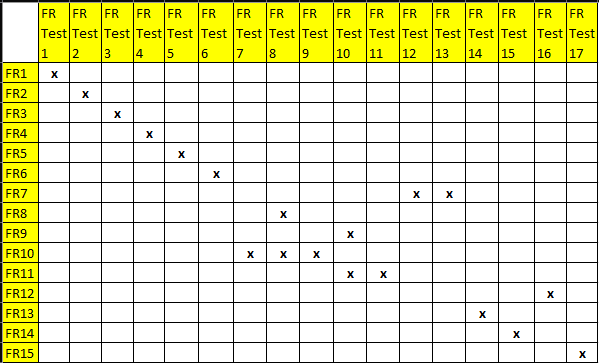
\includegraphics[width=\textwidth]{fr_mat.png}\\
\caption{Functional Requirements and Test Case Traceability Matrix}
\end{figure}


\begin{figure}[!h]
\centering
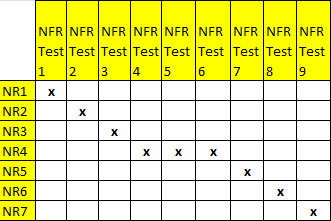
\includegraphics{nfr_mat.png}\\
\caption{Non-Functional Requirements and Test Case Traceability Matrix}
\end{figure}

\newpage

\section{Unit Test Description}
\textbf{Unit tests will be filled after the system design phase is complete. Please ignore the entire section 6 until the design phase is complete and V\&V plan is revised.}
% \subsection{Unit Testing Scope}
% \subsection{Tests for Functional Requirements}
% \subsubsection{Module 1}
% \subsubsection{Module 2}
% ...


% \subsection{Tests for Nonfunctional Requirements}
% \subsubsection{Module ?}
% \subsubsection{Module ?}

% ...

%\subsection{Traceability Between Test Cases and Modules}

				
\bibliographystyle{plainnat}

\bibliography{../../refs/References}

\newpage

\section{Appendix}

\subsection{Symbolic Parameters}
N/A

\subsection{Usability Survey Questions}

\begin{itemize}
    \item After explanation from the developers, how confident are you able to navigate the system on scale of 1-5? (5 - very confident)
    \item How readable is data from the Data Visualizer from a scale 1-5? (5 - easily readable)
    \item How easy is it to filter to the wanted data points from the Data Visualizer? (5 - very easy)
\end{itemize}

\newpage{}
\section*{Appendix --- Reflection}

The skills required to complete verification and validation for the project will be specific library experience in PyTest and unnittest, dynamic testing knowledge, and static testing knowledge.

For library experience in PyTest and unnittest will be crucial in dealing with tests requiring automated testing to give us immediate feedback without manual interaction for cases like FR 6 and FR Test 14. Without the automated testing libraries, it would take too much time to test manually. 

Dynamic testing knowledge is essential to understand as mentioned before, we will use an automated testing protocol for some of the tests to make it much easier to confirm if core aspects of the system are still functional during iterative implementation.

Static testing knowledge will be required to commit to code reviews to ensure that coding principles are kept throughout the implementation or additional features after the initial implementation has been completed.

The PyTest and unnittest can be learned through either video tutorials or using starter code examples to learn from. The group will begin with starter code examples as we all have had prior experience with these libraries already, if we need more assistance opt to use video tutorials.

Dynamic testing knowledge can be learned through the same suit as the Python libraries are automated testing libraries.

Static testing knowledge can be obtained through online sources or by gaining experience through our capstone supervisors. The group as a whole shall gain knowledge through the means of our capstone supervisors because it is a very lucrative resource that we may not always have access to and the supervisors are knowledgeable on the topic of our project. As a last resort, online resources are always available for us to research. 





\end{document}